\ProvidesFile{chapters/ch-Event_Simulation.tex}

\chapter{Monte Carlo Event Simulation}
In particle physics, completely analytical simulations are far too complicated and computationally expensive to be feasible.
Instead, numerical Monte Carlo (MC) techniques employ a combination of analytical calculations and both probabilistic and phenomenological models to simulate $pp$ collisions, the production, decay, and showering of particles, as well as the detector response.
MC simulations are used to optimize the analysis of data, study the performance of the detector, and to compare the results of experiments to theoretical predictions.
These simulations are not perfect, as they do contain approximations, modeling assumptions, and systematic uncertainties, but they are accurate enough to make per cent precision measurements possible.
A schematic representation of the different steps of MC simulation for $pp$ collisions is shown in figure~\ref{MC_simulation}.
\begin{figure}[!h]
  \begin{center}
    \begin{tabular}{c}
        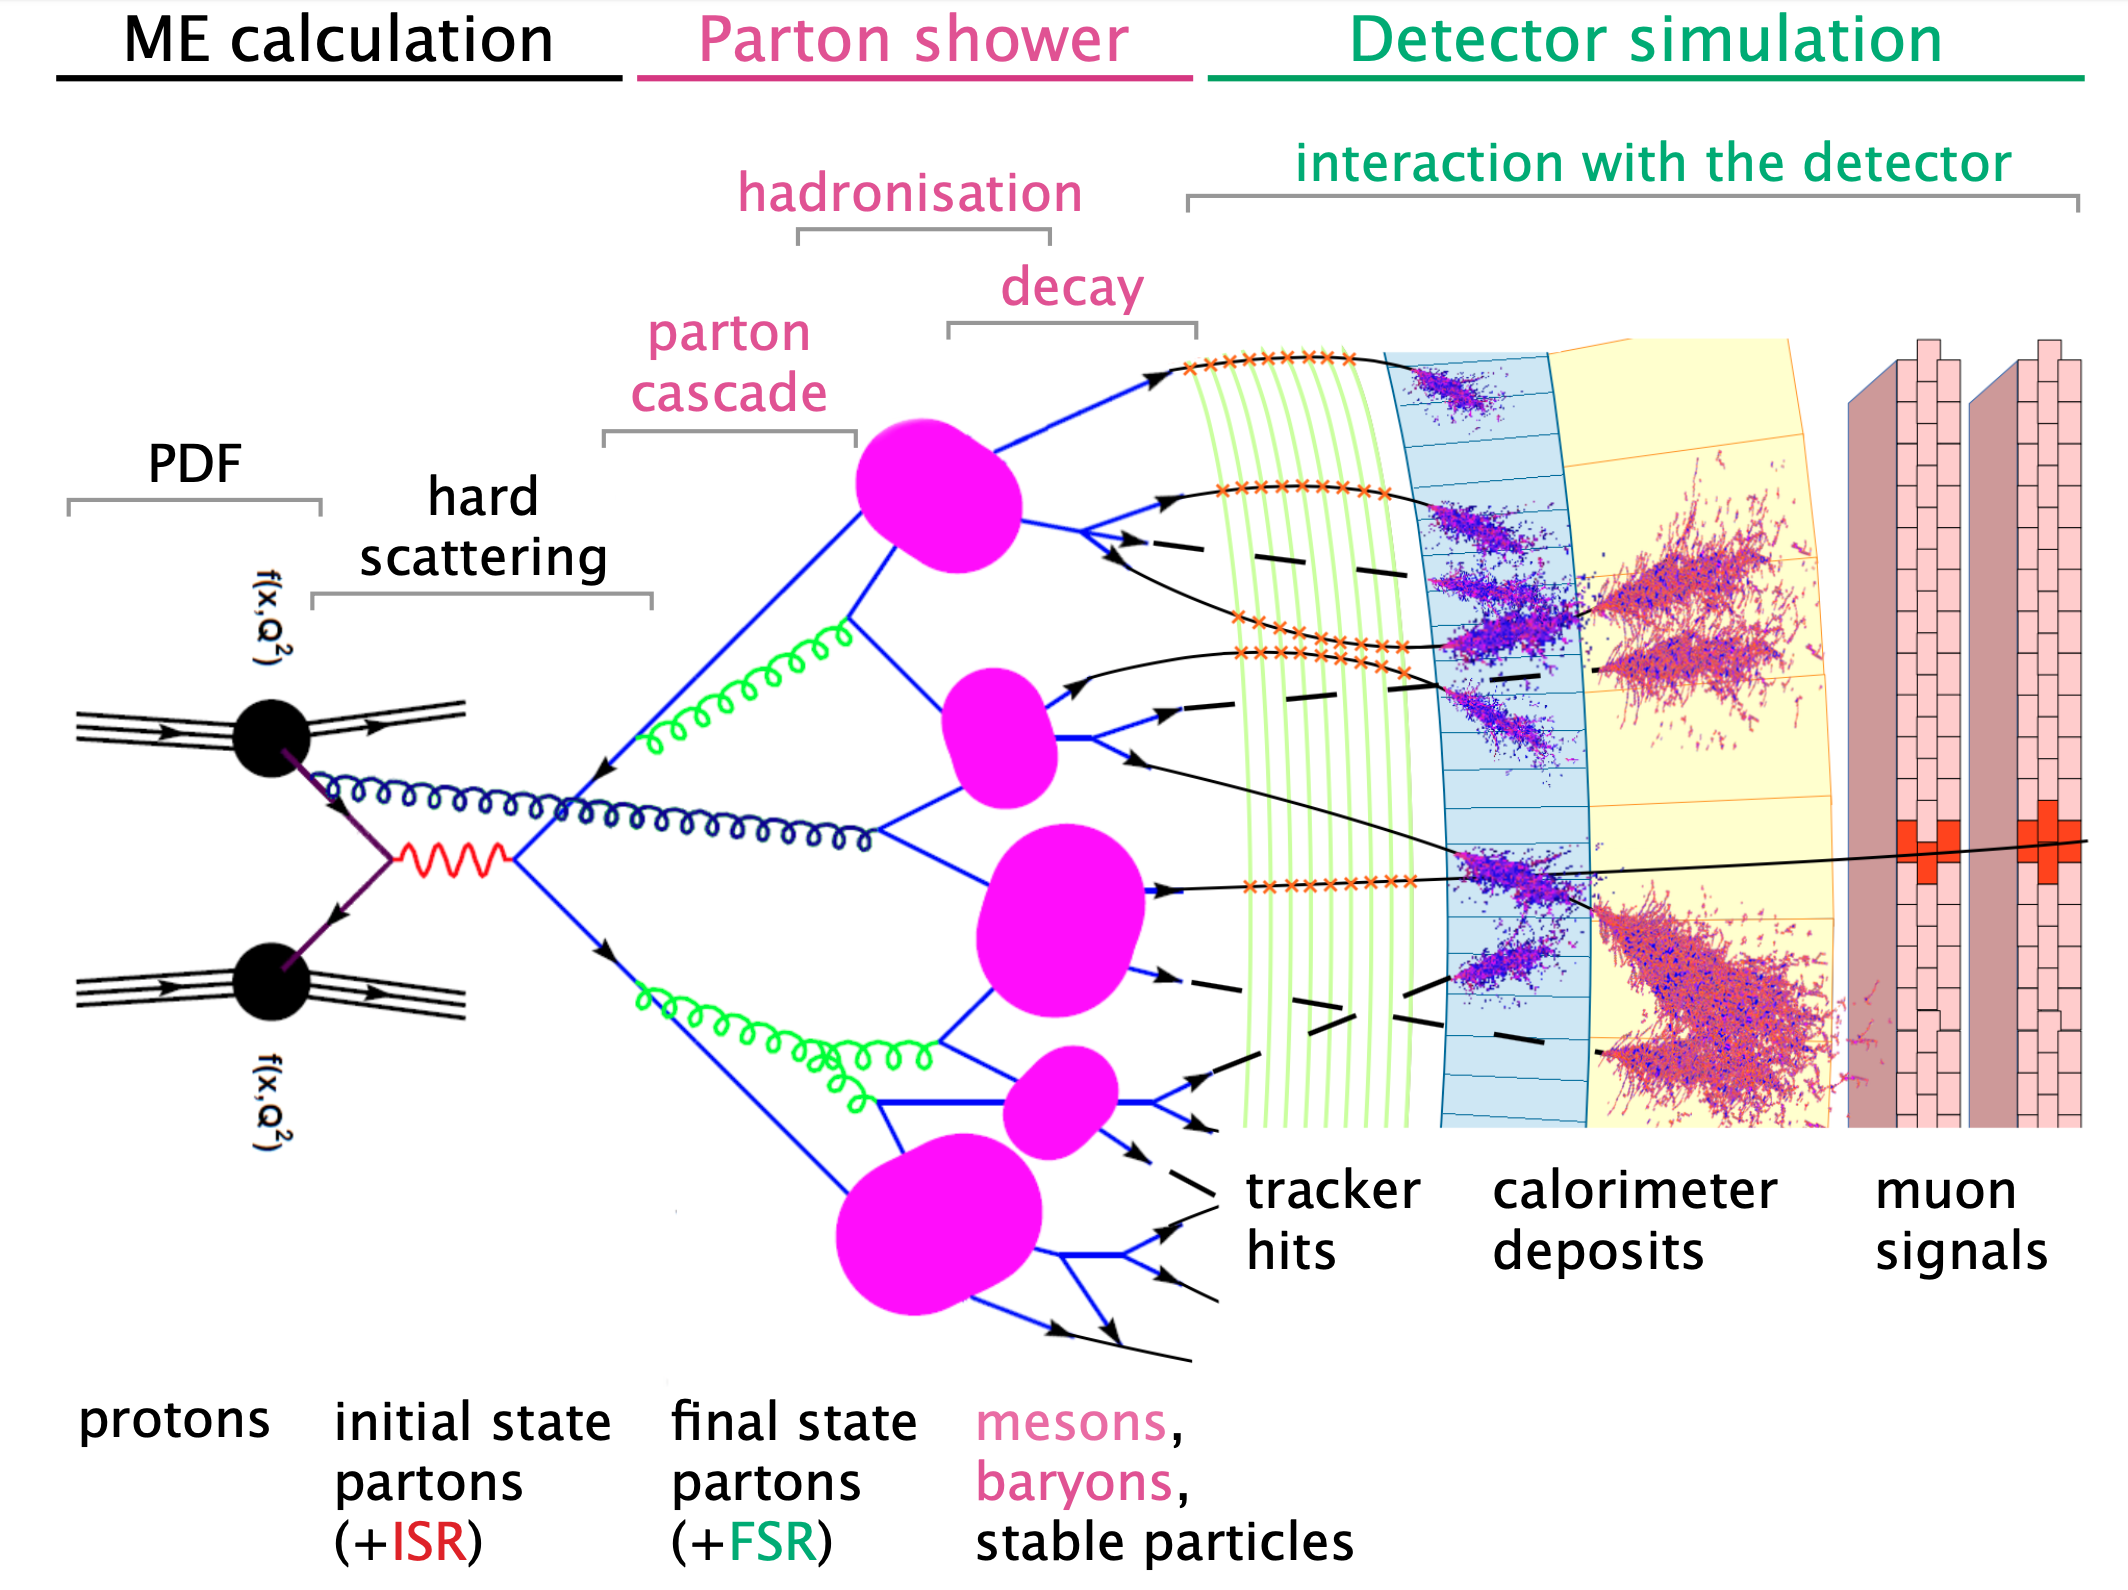
\includegraphics[width=0.9\textwidth]{fig_Event_Simulation/MC_simulation.png}
    \end{tabular}
    \caption{A schematic representation of the different steps of MC simulation for $pp$ collisions~\cite{bartosik}.
            }
    \label{MC_simulation}
  \end{center}
\end{figure}

To minimize statistical uncertainties, MC simulations are usually performed with statistics much higher than in data recorded by the detector, and can be reweighted to match the luminosity of recorded data:
\begin{align}
w = \frac{\mathcal{L} \cdot \sigma_{\text{Process}}}{N_{\text{Gen}}}
\end{align}
where $w$ is the global event weight, $\mathcal{L}$ is the measured integrated luminosity of recorded data, $\sigma_{\text{Process}}$ is the cross-section of the simulated process, and $N_{\text{Gen}}$ is weighted sum of simulated events.

\section{Parton Distribution Functions}
For inelastic $pp$ collisions at the LHC, partons within the proton are at sufficient energies to be asymptotically free, and the hard process can be treated as a direct parton-parton interaction.
Protons are composed of not only three valence quarks, but also gluons and a sea of virtual quarks.
The proton parton distribution functions (PDF), shown in figure~\ref{Parton_Distribution_Functions}, give the probability density $f$ of finding a specific parton within the proton with a certain fraction $x$ of the proton's longitudinal momentum at factorization scale $\mu_F$.
\begin{figure}[!h]
  \begin{center}
    \begin{tabular}{c}
        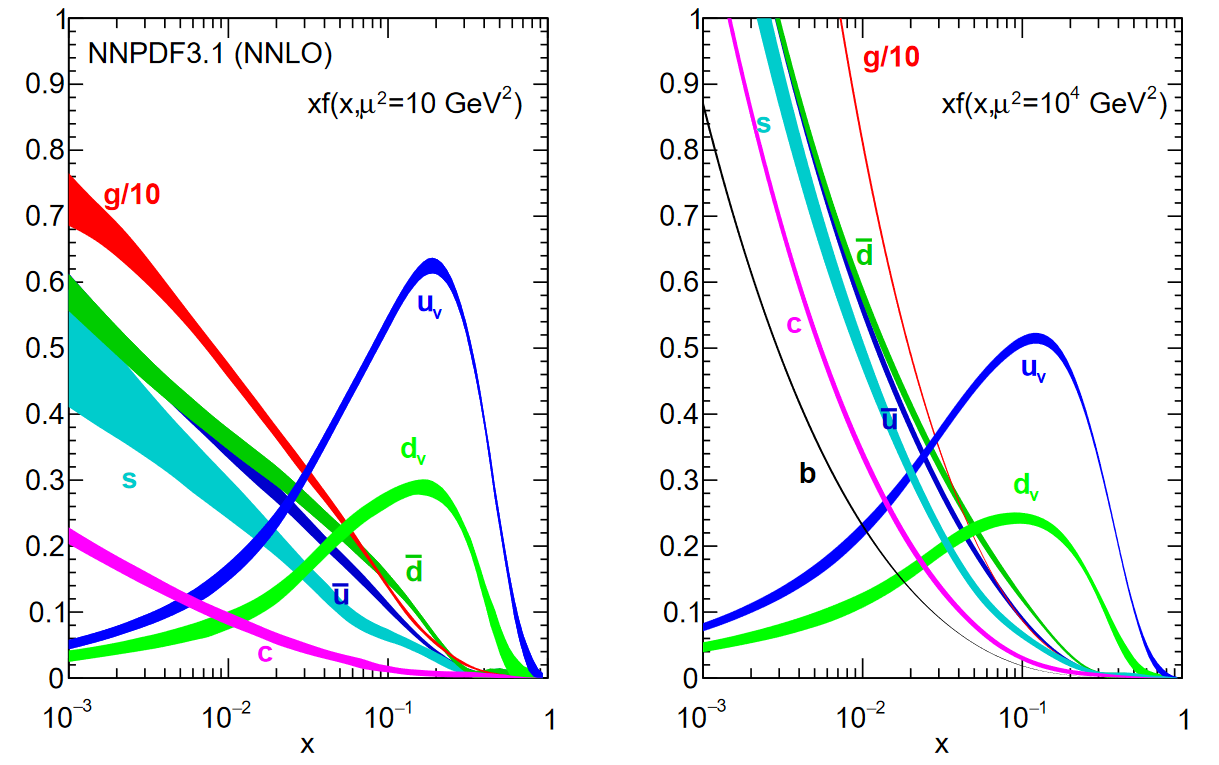
\includegraphics[width=0.80\textwidth]{fig_Event_Simulation/Parton_Distribution_Functions.png}
    \end{tabular}
    \caption{The proton PDF gives the probability density $f$ of finding a specific parton within the proton with a certain fraction $x$ of the proton's longitudinal momentum.
    Shown for scales $\mu_F = \SI{3.1}{\GeV}$ (Left) and at $\mu_F = \SI{100}{\GeV}$ (Right), according to the NNPDF collaboration~\cite{Ball:2267455}.
            }
    \label{Parton_Distribution_Functions}
  \end{center}
\end{figure}
The PDF cannot be calculated from first principles, so it has to be determined experimentally from fitting a combination of data from different types of deep inelastic scattering and hadron collision measurements.
This measurement uses the NNPDF3.1 set of PDFs.

\section{Matrix Element Calculation and Production Cross-section}
A hard interaction is an event is a process in which heavy objects are created or a large momentum transfer occurs.
For hard parton scattering processes at high energy proton colliders $\alpha_S << 1$, so partonic cross sections can be expanded in a power series expansion of $\alpha_S$ and be calculated in fixed-order perturbation theory. 
Perturbative calculations to accuracies $\mathcal{O}(\alpha^2_S)$, $\mathcal{O}(\alpha^3_S)$, and $\mathcal{O}(\alpha^4_S)$ are referred to as leading-order (LO), next-to-leading-order (NLO), and next-to-next-to-leading-order (NNLO), respectively.
The partonic cross-sections are convoluted with the proton PDFs to obtain $pp$ collision production cross-sections~\cite{BUCKLEY2011145}.
The cross-section or the scattering process $IJ \rightarrow X$ can be expressed as:
\begin{align}
\sigma_{IJ \rightarrow X}(s, \mu_F, \mu_R) = \sum_{i, j = g, q, \bar{q}}^{} \int_{0}^{1} \mathrm{~d} x_i \mathrm{~d} x_j f_{\sfrac{i}{I}}\left(x_i, \mu_F^2\right) f_{\sfrac{j}{J}}\left(x_j, \mu_F^2\right) \cdot \hat{\sigma}_{i j \rightarrow X}\left(\hat{s}, \mu_F, \mu_R, \alpha_S\right) \\
=\sum_{i, j=g, q, \bar{q}} \int_{0}^{1} \mathrm{~d} x_i \mathrm{~d} x_j \int \mathrm{~d} \Phi_X f_{\sfrac{i}{I}}\left(x_i, \mu_F^2\right) f_{\sfrac{j}{J}}\left(x_j, \mu_F^2\right) \cdot \frac{1}{2 \hat{s}}\left\vert \mathcal{M}_{i j \rightarrow X}\right\vert^2\left(\Phi_X, \mu_F, \mu_R, \alpha_S\right)
\label{ttbar_crosssection}
\end{align}
where $i(j)$ are the parton constituents of proton $I(J)$, $f_{{\sfrac{i}{I}}({\sfrac{j}{J}})}$ are the parton $i(j)$ PDF of proton $I(J)$, $x_{i(j)}$ are the parton $i(j)$ momentum fraction of proton $I(J)$, $\mu_F$ is the factorization scale, $\mu_R$ is the renormalization scale, $\sigma_{i j \rightarrow X}$ are the exclusive partonic cross-sections for $X$ production, $\hat{s} = s \cdot x_i \cdot x_j$ is the squared center-of-mass energy of the parton collision, \beamenergy is the center-of-mass energy of the proton-proton collision, $\alpha_S$ is the coupling constant of the strong interaction, $\Phi_X$ is the final state phase space, and $\left\vert \mathcal{M}_{i j \rightarrow X}\right\vert^2$ is the matrix element (ME) squared.
The factorization scale $\mu_F$ is conventionally set to the energy scale of the high-energy protons in the collision.
The renormalization scale $\mu_R$ is the arbitrarily chosen high-energy cutoff for the renormalization procedure, used in perturbation theory to separate divergences from higher order corrections.
The ME are calculated by summing over the contributions from the relevant fix-order Feynman diagrams ($\mathcal{M}_{i j \rightarrow X}=\sum_k \mathcal{F}_{i j \rightarrow X}^{(k)}$), summing over the outgoing spin and color quantum numbers, and averaging over the incoming ones.
At LO, ME calculations only include the interaction between incoming partons, but higher order ME calculations will additionally include real emission and virtual loop corrections.
The real emission corrections correspond to radiated partons, which are classified as initial state radiation (ISR) and final state radiation (FSR) depending on whether they are emitted by the incoming or outgoing particles.
This measurement uses the Positive Weight Hard Event Generator v2 (\Powheg) event generator, which perform ME calculations with NLO accuracy and accounts for polarizations in \ttbar production and top quark decays.

\section{Parton Shower}
Parton shower (PS) models account for higher order QCD and QED radiative emissions beyond the accuracy of fixed order perturbative approximations.
Showers of outgoing partons are created as partons radiate gluons and gluons radiate other gluons or produce $q\bar{q}$ pairs.
In this measurement, the PS is modelled using (\Pythia).
In \Pythia\ the radiative emissions are modeled as a Markov chain, where each emission is treated as independent, with the probability of an additional emission being determined by the splitting functions and the kinematics of the partons involved~\cite{pythia8.3}.
The algorithm continues to iteratively split the partons in a cascade of emissions until they reach an energy scale where perturbation theory breaks down.

A matching procedure is used to avoid double-counting radiative emissions from the ME calculation and the PS models~\cite{StefanoFrixione_2007}.
In \Powheg, the $h_{damp}$ parameter controls the matching procedure by modifying the scale at which radiative emissions from the PS are discarded in favor of the ME calculations.
Lower (higher) values of $h_{damp}$ result in softer (harder) radiated emissions and less (more) events with high \pT jets.

For $pp$ collisions, besides the parton interaction in the hard process, the remaining constituent partons of the colliding protons, referred to as the beam-beam remnants (BBR), can also interact.
These multiple parton interactions (MPI) can produce additional independent scattering processes that contribute to the underlying event (UE).
PS models in event generators have a adjustable parameters to control the behavior of event modeling, and a set of these parameters, which has been adjusted to better fit some aspects of the data, is referred to as a UE tune~\cite{Sirunyan:2669320}.
The CP5 UE tune was chosen for all simulated samples for this measurement.

\section{Hadronization}
Hadronization is the direct consequence of color confinement and the running of $\alpha_S$ at low energy scales where QCD is non-perturbative.
As non-perturbative QCD is unsolved, hadronization is simulated using phenomenological models that describe the process of forming colorless hadrons from quarks and gluons.
In \Pythia, it is based on the Lund string model, which assumes that the potential energy of color charge dipole fields grows linearly ($V(r) = \kappa r$ with $\kappa \approx \SI{1}{\GeV \per \femto \m}$) with the separation of the charges~\cite{SJOSTRAND2015159}.
As color charges ($q$ and $\bar{q^\prime}$) separate, the potential energy increases beyond the threshold that the color flux tube snaps and a new color charge pair ($q^\prime$ and $\bar{q^\prime}$) emerges.
After the snap, the system consists of two separate color charge dipole fields ($q\bar{q^{\prime\prime}}$ and $q^{\prime\prime}\bar{q^\prime}$).
Further snaps continue until the potential energy of the tubes are not sufficient to produce new color charge pairs.

In these models, individual partons do not hadronize independently, but rather colour-connected systems of partons hadronize collectively~\cite{BUCKLEY2011145}.
The scenario in which color lines connecting different partons may rearrange themselves before the formation of final hadrons is referred to as color reconnection (CR).
To more accurately describe the data, phenomenological CR models are used to simulate color-flow.
\Pythia\ uses a MPI-based CR scheme in which there is a probability that the partons of the lower-\pT proton are added to the strings defined by the higher-\pT proton in such a way as to give the smallest total string length.

\section{Detector Response}
The interaction of the MC generated final state particles with the CMS detector are simulated with the GEometry ANd Tracking (\Geant v10.4.3) toolkit.
\Geant\ divides the the trajectory of particles traversing the detector into small, finite steps and calculates the probability that the particles will interact with the material in the detector based on their properties and the properties of the material they are passing through~\cite{AGOSTINELLI2003250}.
A complete set physics models for the electromagnetic, strong and weak interactions are included in \Geant.
If an interaction occurs, \Geant\ calculates the resulting energy deposition, generates any secondary particles that are produced, and simulates the response of the readout electronics and trigger system including the effects of noise and other sources of background.
To provide an accurate simulation, \Geant\ uses a detailed description of the detector geometry and materials, calibrations, and electronics performance including dead channels.
Experimental data is used to parameterize detector response and validate the simulation~\cite{Bayatian:922757}.
The collection of \Geant-simulated detector responses for an event is stored in the raw CMS event data model (EDM) format and can be reconstructed exactly as actual events recorded by the CMS detector.